%%%%%%%%%%%%%%%%%%%%%%%%%%%%%%%%%%%%%%%%%%%%%%%%%%%%%%%%%%%%%%%%%%%%%%%
\chapter{Introduction}
\label{cha:introduction}
Software developers spend more time reading source code than writing. Lowering the cognitive burden to understand the presented program sources is a key factor to increase productivity. \\

%DSLs 
Presenting the program specific to the qualifications and domain of the reader helps lowering the entrance barrier. Domain specific languages help non software developers to be integrated in the developing process and help them understanding and correcting the program. Embedded or internal domain specific languages have a low entry barrier, but lack the ability for visual editing and domain specific feedback. Because they are embedded in a host language, internal domain specific languages have to follow their syntax constraints. Internal domain specific languages are source code, which is often repelling for non software developers. External domain specific languages are flexible in notation and user guidance, but development and maintenance costs are higher. Additional tools or an additional tool chain is required and changes in the language are much more effort. External domain specific languages are integrated in the runtime either by using their result as a configuration for an interpreter or by generating source code. Interpreting the word of a language completely decouples the external domain specific language from the source code. With the generative approach, generated source code from the domain specific description coexistence in general side by side with hand written code. External languages in general are no general purpose languages, otherwise their complexity goes towards the target language making their development expensive and the target language obsolete. Coexistence of general and hand written code is not consensual, because source code generation is unidirectional and overwriting in most cases. Integration with hand written code must be designed carefully and it is impossible, incremental development is hindered and synchronicity is not maintained. No fluent transition from internal to external domain specific languages is possible.   

% Modern IDEs
Modern integrated development environments (IDEs) are designed to maximize the productivity of its user. Thus, is leverage the plain source code representation of the source code by processing it and providing a comprehensive view on the program description. They provide navigation and refactoring based on computed meta data, allow the user to customize the view to a certain extend and manipulate the source code by predefined actions. The source code is the central description of the program, but visual viewing, refactoring and processing of the textual input is usually done on an abstract data structure gained by parsing the textual input. The parsing is mainly based on a context free grammar for a textual language. 

% Modeling
Modeling tools for visual languages on the other hand are strongly based on the model view controller pattern and thus separate the notation for a language with their abstract description. The well known Unified Modeling Language 2 (UML2) uses a model to formally describe the abstract syntax of a language and constraints to describe its static semantics. These models of languages form the common denominator for tools and frameworks for working with the described language. General use cases are model transformation, model presentation in textual or graphical manner, model validation, model persistence and so on. These models integrate tools which are able to create, present and process instances of a described language, they form the common ground for component oriented language workbenches. 
%Bridging

% Model <-> Text
Several tools \footnote{\raggedright XText, Textual Editing Framework, EMFText} already bridge the gap between the description of a language by a context free grammar and by models. They require a full textual representation of a model element and its content do not allow the user to select alternative textual presentations of semantic equivalent element. Projectional editors like Meta Programming Systems offer form based textual views on data structures, whose design approach is 	 predestined to show just parts of the model or to present certain model elements differently. Projectional editors enforce a special the user guidance, which is more restrictive to free textual editing. Additionally, they require continuous structural correctness while editing, which enforces the user to make edits in steps which are at least structurally correct. This contradicts well-known editing behavior, where users create several incorrect intermediate states of a document to reach the desired, correct state. Abandoning this editing behavior restricts the user in his familiar work flow. It requires not only him to learn the model manipulating tool, but also to learn and to switch to another editing paradigm. 

This thesis started from the basic idea to leverage internal domain specific languages with domain specific notation and domain specific manipulation facilities interchangeable. This requires to mix textual and graphical notations interchangeable and integrate the editor in the word as if it was part of it. So the data in place of the editor has to be part of a word. This word should be in language described by a context free grammar.
 
%%% TODOSSSSSSSSSSSSSSSSSSSSSSSSSSSSSSSSSSSSSSSSSSSSSSSSSS 
\todo{DSLs should integrate in IDE}

\todo{integrate}
``An attractive goal is to provide support for simultaneous editing of textual and graphical elements for any language.''\cite{EMP}
\todo{current solutions replace view elements instead of change property}
\todo{name it Impedance mismatch}

\todo{closed under composition}

\textbf{
"Not only is no single representation best for all kinds of programs, no single representation is one representation even best for all tasks involving the \emph{same}  program. " \cite{Petri} }



\section{Research Objective}
The central \emph{questions} of this thesis are:
\begin{itemize}
	\item How are different, interchangeable textual representations of the semantically same abstract language element are in general possible?
	\item How can graphical editors be integrated in a text, so that the text is still a word of the language described by a context free grammar?
	\item Which granularity of integration is possible if different editors are unknown at design time of the context free grammar?
\end{itemize}

This thesis uses an abstract notion of graphical editors in which the type of editor, its position in the character stream and a proper data source is sufficient to facilitate their deployment.

\todo{Constraint thesis that errors are not specially considered?}

% check >>>>>>>>>>>>>>>>>>>>>>>


%%%%%%%%%%%%%%%%%%%%%%%%%%%%%%%%%%%%%%%%%%%%%%%%%%%%%%%%%%%%%%%%%%%%%%%
\section{Outline}
% Outline Solution
The general idea of the presented solution combines three simple concepts:
\begin{itemize}
	\item The use of private characters as a unique key for a map. The value of the map is an object, thus a single character can be resolved to an arbitrary data structure.
	\item The parse tree is a tree data structure. If a part of the tree produced by a token sequence is saved in a single token, that token is a valid substitute for that tree part.
\end{itemize}
These two already allow to operate on the parse tree part in the map.
\begin{itemize}
	\item A parse tree constructor, which constructs a parse tree from an abstract syntax tree and is extensible, to assign types to and to skip parse tree construction for invisible elements. This allows the graphical editor to use the abstract syntax tree as data source directly. 
\end{itemize}

Figure \ref{ConceptFigure} shows the conceptional overview. 

% Outline thesis
The results of the work were achieved by an argumentative deductive approach. 



Definitions contain formal definitions for wide spread concepts of computer science. Basics lay the common ground for further explanations. An available solutions of creating EMF models from text is used to present the current state. The concepts XText in regards to this thesis are explained and discussed to gain problem awareness and to expose room for improvement. \todo{Present Notation model, discuss resource impl. Etc.}
\todo{all of them}

\begin{figure}
\centering
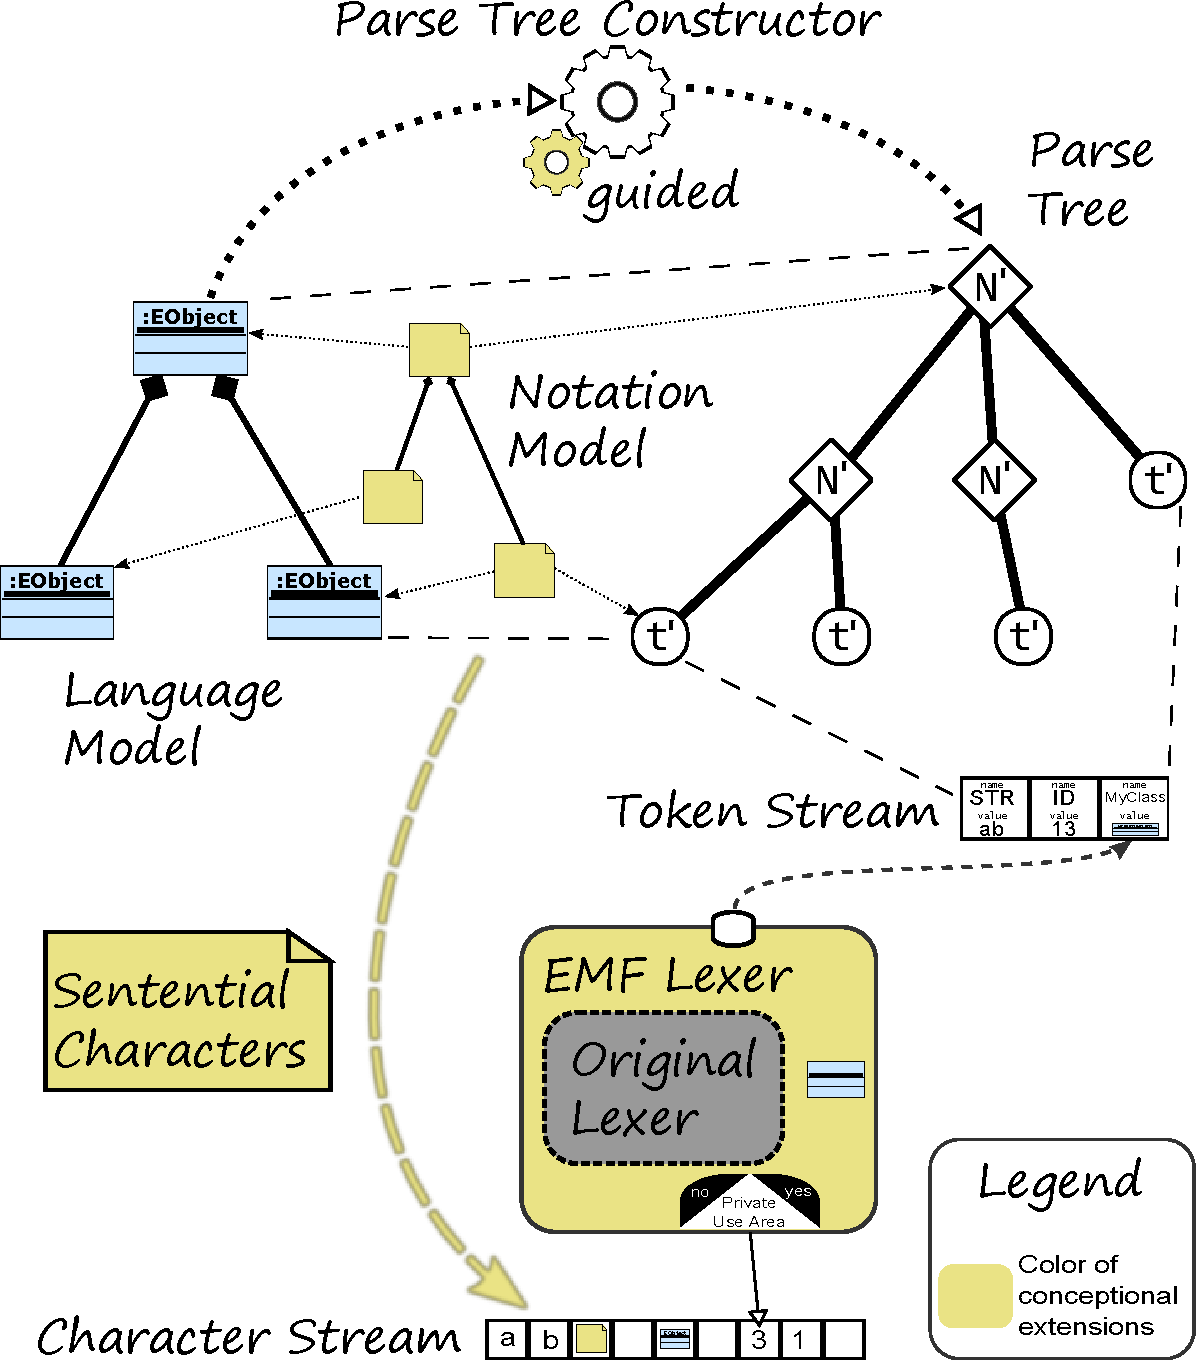
\includegraphics[scale=0.75]{gfx/ex/Concept} 
\caption{Conceptual Overview}
\label{ConceptFigure}
\end{figure}